\documentclass[12pt]{article}
\usepackage{fullpage}
\subsectionfont{\fontfamily{phv}\fontsize{13pt}{13pt}\selectfont}
%\newcommand{\var}[1]{\mathit{#1}}
\usepackage[margin=1cm]{geometry}
\usepackage{amsmath}
\usepackage{graphicx}

\usepackage{listings}



\begin{document}


\begin{titlepage}


\newcommand{\HRule}{\rule{\linewidth}{0.5mm}} % Defines a new command for the horizontal lines, change thickness here

\center % Center everything on the page
 
%----------------------------------------------------------------------------------------
%	HEADING SECTIONS
%----------------------------------------------------------------------------------------



\HRule \\[0.4cm]
{ \huge \bfseries Phase 2}\\[0.4cm] % Title of your document
\HRule \\[1.5cm]
 
\begin{minipage}{0.4\textwidth}
\begin{center} \large
Programming on the Web\\
CSC309H1, Winter 2015\\
\today
\end{center}
\end{minipage}


\vfill % Fill the rest of the page with whitespace


Cody Rosevear, c3roseve\\
999499332\\
\\
Denis Marchin, g3dmarch\\
999061009\\
\\
Farzad Hemmati, c3hemmat\\
999964953\\
\\


Akira Kakkar, g3fol\\
999825541\\
\\



\end{titlepage}
\newpage
\section*{Description}
\begin{enumerate}
\item[1.] Feature and Functionality Specification
\begin{figure}[ht!]
\centering
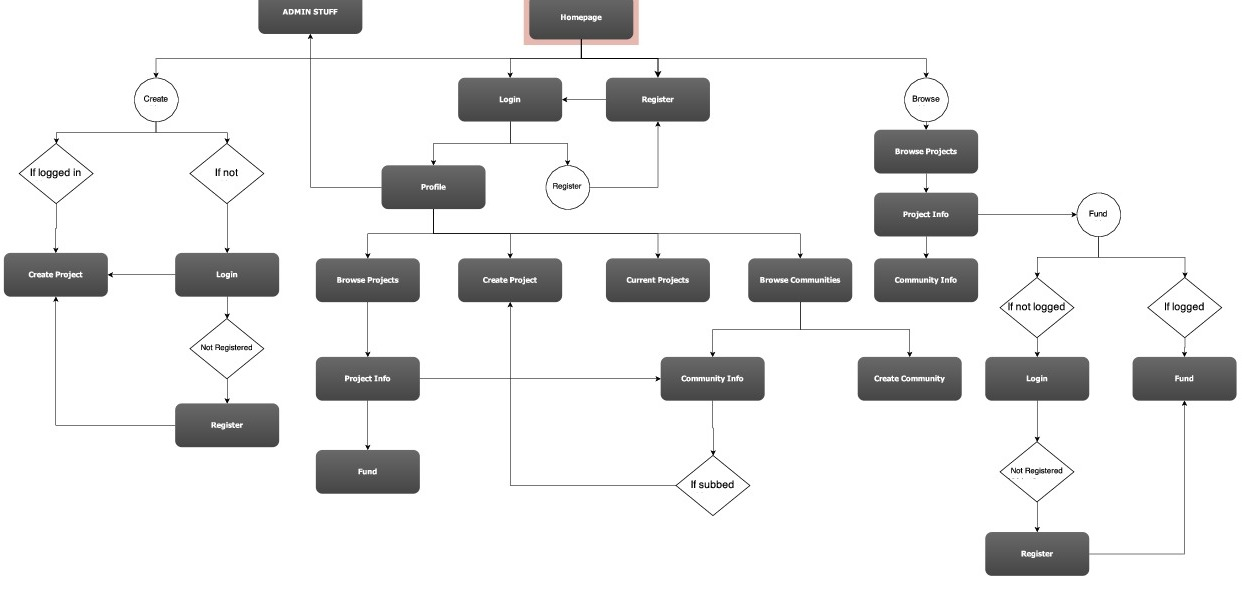
\includegraphics[width=200mm]{flowchart.jpg}
\caption{Website Flowchart \label{overflow}}
\end{figure}

\item[2.] Project Plan 
\item[3.] Software Architecture and High-level Design
\begin{figure}[ht!]
\centering
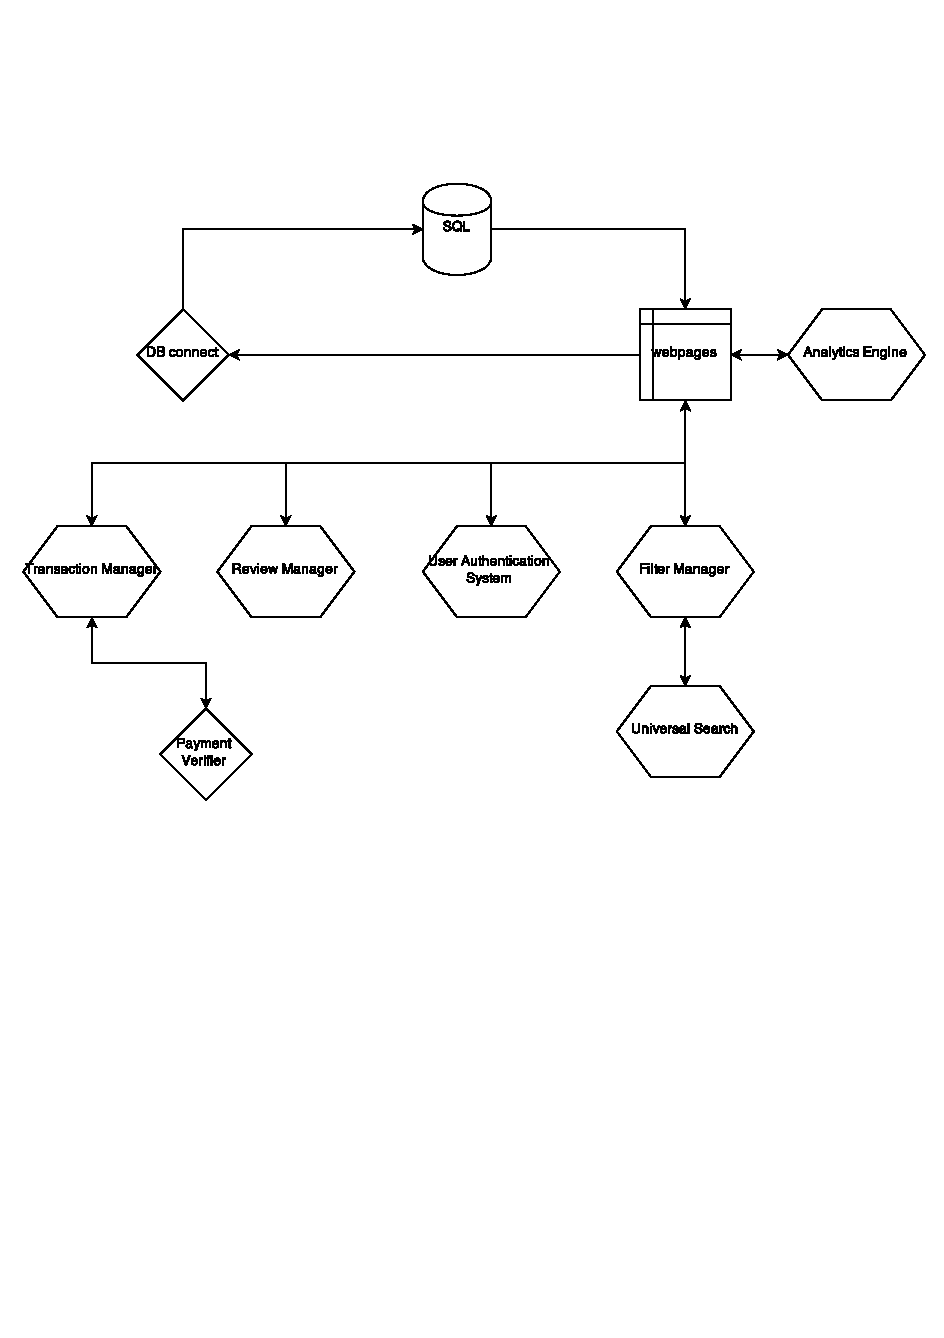
\includegraphics[width=200mm]{swag.pdf}
\caption{Website Flowchart \label{overflow}}
\end{figure}

\item[4.] Information Representation
\item[5.] Test Strategy and Test Plan	
\end{enumerate}
\end{document}


